\documentclass[xcolor={dvipsnames},aspectratio=169,10pt]{beamer}
\usetheme{mx}
\usepackage{graphicx}
\graphicspath{{figures/}}
%\input{preamble.tex}

\title{  
%Prototyping Good AL/ML practices for Medical Image Synthesis
Good practices in AI/ML for Medical Image Synthesis %Fri 19 May 11:54:10 BST 2023
} 
\subtitle{
The deep learning and computer vision Journal club \\
UCL Centre for Advance Research Computing
}

\author{
Harvey Mannering, Sofia Mi\~nano, and  \\ 
{\bf Miguel Xochicale} (\faTwitter @\_mxochicale  \faGithub @mxochicale)
}
\date{
1st of June 2023
%\today
}
\institute{
Advanced Research Computing Centre and WEISS at University College London 
}

\githubrepository{https://github.com/mxochicale/medisynth}
\begin{document}
\maketitle

\begin{frame}
\frametitle{Table of Contents}
    \tableofcontents
\end{frame}


\section{Medical Image Synthesis}
\subsection{Background}
\begin{frame}
  \frametitle{Table of Contents}
  \tableofcontents[currentsection]
\end{frame}



%%%%%%%%%%%%%%%%%%%%%%%%%%%%%%%%%%%%%%%%%%%%%%%%%%%%%%%%
{
\paper{
Yi X., Walia E., and Babyn P., "Generative adversarial network in medical imaging: A review." Medical image analysis 58 (2019): 101552.
}

\begin{frame}{Generative adversarial network in medical imaging}{}
      \begin{figure}
        \centering
        \includegraphics[width=1.0\textwidth]{gans-in-medimg-applications/outputs/drawing-v00}
        % \caption{The sonographer-probe-patient control system}
      \end{figure}
\end{frame}
}

%%%%%%%%%%%%%%%%%%%%%%%%%%%%%%%%%%%%%%%%%%%%%%%%%%%%%%%%
{
\paper{
Yi X., Walia E., and Babyn P., "Generative adversarial network in medical imaging: A review." Medical image analysis 58 (2019): 101552.
}

\begin{frame}{Generative adversarial network in medical imaging}{}
      \begin{figure}
        \centering
        \includegraphics[width=1.0\textwidth]{gans-in-medimg-task-modalities-papers/outputs/drawing-v00}
        % \caption{The sonographer-probe-patient control system}
      \end{figure}
\end{frame}
}




\subsection{Methods}

%%%%%%%%%%%%%%%%%%%%%%%%%%%%%%%%%%%%%%%%%%%%%%%%%%%%%%%%
{
\paper{
Yi X., Walia E., and Babyn P., "Generative adversarial network in medical imaging: A review." Medical image analysis 58 (2019): 101552.
}

\begin{frame}{GANs background}
% \BigSizeFont
\begin{itemize}

\item Challenges in optimisitation
    \begin{itemize}
    \item Balance and stabilisation for training of $G$ and $D$, 
    \item Mode collapse (limiting learning to few modes)
    \end{itemize}

\item Varians of GANS
    \begin{itemize}
    \item Varying objective of $D$
    \item Varying objective of $G$
    \item Varying arquitecture
    \end{itemize}

\end{itemize}

\end{frame}
}



%%%%%%%%%%%%%%%%%%%%%%%%%%%%%%%%%%%%%%%%%%%%%%%%%%%%%%%%
{
\paper{
Yi X., Walia E., and Babyn P., "Generative adversarial network in medical imaging: A review." Medical image analysis 58 (2019): 101552.
}

\begin{frame}{Generative adversarial network in medical imaging}{}
      \begin{figure}
        \centering
        \includegraphics[width=1.0\textwidth]{gans-in-medimg-variants/outputs/drawing-v00}
        % \caption{The sonographer-probe-patient control system}
      \end{figure}
\end{frame}
}






\subsection{Applications}


\section{Good practices in AI/ML and checklists}
\begin{frame}
  \frametitle{Table of Contents}
  \tableofcontents[currentsection]
\end{frame}

%\subsection{checklist for artificial intelligence in medical imaging (CLAIM)}

\subsection{FDA-approved AI-based Medical Devices}

%%%%%%%%%%%%%%%%%%%%%%%%%%%%%%%%%%%%%%%%%%%%%%%%%%%%%%%%
{
\paper{
Benjamens S., Dhunnoo  P. and  Mesk\'o B. The state of artificial intelligence-based FDA-approved medical devices and algorithms: an online database. npj Digit. Med. 3, 118 (2020).
}
\begin{frame}{
FDA-approved AI-based Medical Devices
}{
%(2019-2021) @ KCL
}
      \begin{figure}
        \centering
        \includegraphics[width=1.0\textwidth]{fda-approved-ai-based-med-devs/outputs/drawing-v00}
        % \caption{The sonographer-probe-patient control system}
      \end{figure}
\end{frame}
}







\subsection{Quality Systems and Good Machine Learning Practices (GMLP) by FDA}
%%%%%%%%%%%%%%%%%%%%%%%%%%%%%%%%%%%%%%%%%%%%%%%%%%%%%%%%
{
\paper{
%\url{https://www.fda.gov/files/medical%20devices/published/US-FDA-Artificial-Intelligence-and-Machine-Learning-Discussion-Paper.pdf}
US-FDA-Artificial-Intelligence-and-Machine-Learning-Discussion-Paper
}
\begin{frame}{
Regulatory Framework for Modifications to \\
(AI/ML)-Based Software as a Medical Device (SaMD)
}{
%(2019-2021) @ KCL
}
      \begin{figure}
        \centering
        \includegraphics[width=1.0\textwidth]{goodALMLFDA/outputs/drawing-v00}
        % \caption{The sonographer-probe-patient control system}
      \end{figure}
\end{frame}
}

%%%%%%%%%%%%%%%%%%%%%%%%%%%%%%%%%%%%%%%%%%%%%%%%%%%%%%%%
{
\paper{
Rajpurkar, Pranav, and Matthew P. Lungren. "The Current and Future State of AI Interpretation of Medical Images." New England Journal of Medicine 388, no. 21 (2023): 1981-1990.
}
\begin{frame}{
Checks for AI Systems in Radiology
}{
%(2019-2021) @ KCL
}
      \begin{figure}
        \centering
        \includegraphics[width=1.0\textwidth]{ai-interpreation-of-medical-images/outputs/drawing-v00}
        % \caption{The sonographer-probe-patient control system}
      \end{figure}
\end{frame}
}




\input{content-tex/ultrasound-image-synthesis}
\section{Takeaways}
\begin{frame}
  \frametitle{Table of Contents}
  \tableofcontents[currentsection]
\end{frame}

%%%%%%%%%%%%%%%%%%%%%%%%%%%%%%%%%%%%%%%%%%%%%%%%%%%%%%%%
{
%\paper{}


\begin{frame}{Key takeaways}
% \BigSizeFont
\begin{itemize}
\item Introduction to Medical Image Synthesis 
    \begin{itemize}
    \item Modalities, applications and publications
    \item Generative learning trilemma (GANs, VAEs and diffusion models)
    \end{itemize}

\item Good software practices by FDA
    \begin{itemize}
    \item Approved FDA AI-based Medical Devices
    \item Good ML/AI Practices 
    \end{itemize}

\item Fetal ultrasound imaging synthesis 
    \begin{itemize}
    \item Small datasets of US Imaging (healthy participants)
    \item Diffusion super resolution GAN architecture
    \item Quality assessment of synthesised images with FID 
    \end{itemize}

\item Future work
    \begin{itemize}
    \item Visual Turing Assessment (Grading Quality Control)
    \item Unsupervised medical anomaly detection
    \end{itemize}

\end{itemize}

\end{frame}
}



% \section{Q.A.}
% \begin{frame}
%   \frametitle{Table of Contents}
%   \tableofcontents[currentsection]
% \end{frame}

% %%%%%%%%%%%%%%%%%%%%%%%%%%%%%%%%%%%%%%%%%%%%%%%%%%%%%%%%
% {
% %\paper{}
% \begin{frame}{Thanks}{Miguel Xochicale, PhD (\faTwitter @\_mxochicale  \faGithub @mxochicale)}
%
% \BigSizeFont
% \begin{center}
%     Q.A.
% \end{center}
% \end{frame}
% }




\maketitle
\end{document}
